\documentclass{beamer}
\usetheme[numbering=fullbar,%nofirafonts
]{focus}
\definecolor{main}{RGB}{92, 138, 168}
\definecolor{background}{RGB}{255,255,255}
%\usefonttheme{serif}
\usepackage{pifont}
\usepackage{tcolorbox}
\usepackage{tikz}
\usepackage[cache]{minted}
\usetikzlibrary{positioning,shapes,fit,calc}
\usepackage{natbib}
\usepackage{amsmath,amsthm,thmtools,array,xspace}
\usepackage{stmaryrd}
\usepackage{subfig}
\usepackage{graphicx}
% \input{tikzmacros}
%% \usetikzlibrary{%
%% decorations.fractals,%
%% decorations.shapes,%
%% decorations.text,%
%% decorations.pathmorphing,%
%% decorations.pathreplacing,%
%% decorations.footprints,%
%% decorations.markings,%
%% shadows}

\setminted[Coq]{fontsize=\footnotesize}

\tikzset{
  invisible/.style={opacity=0},
  visible on/.style={alt={#1{}{invisible}}},
  alt/.code args={<#1>#2#3}{%
    \alt<#1>{\pgfkeysalso{#2}}{\pgfkeysalso{#3}} % \pgfkeysalso doesn't change the path
  },
}
\newcommand{\ttl}[1]{{\large \textbf{#1}}}
\definecolor{myorange}{RGB}{255,123,21}
\definecolor{myblue}{RGB}{51,153,255}
\definecolor{mygreen}{RGB}{56,200,31}
\tikzstyle{mem}=[rectangle, draw=black, minimum size=8mm, 
inner sep=3pt, thick, rounded corners, fill=none, opacity=1]

\tikzstyle{program}=[
        rectangle, draw=black, thick, fill=yellow!15,
        inner sep = 2mm]
\tikzstyle{obsline}=[->, dashed, thick]

\title{Itauto\\ an Extensible Intuitionistic\\ SAT/SMT solver  }
  \author{F. Besson}
%\titlegraphic{}
\institute{Celtique/Inria/Univ Rennes}
\date{Mars 2021}

\newcommand*\circled[1]{\tikz[baseline=(char.base)]{
    \node[shape=circle,draw,inner sep=1pt, thick] (char) {\textbf{#1}};}}

\newmintinline[icoq]{Coq}{}
\newcommand{\mcoq}[1]{\mbox{\icoq{#1}}}
\newcommand{\xmark}{\ding{55}}%

\begin{document}
%\titlepage{}

\begin{frame}
  \maketitle
\end{frame}

\begin{frame}{Yet another SAT solver?}
  \begin{itemize}
  \item \icoq{tauto}: historic decision procedure for IPL\footnote{IPL = Intuitionistic Propositional Logic} 
  \item \icoq{rtauto}: reflexive verifier for IPL
  \item \icoq{intuition tac}: calls \icoq{tac} at the leaf of proof search
  \item \icoq{lia}: linear arithmetics + classic  connectives
  \end{itemize}

  \medskip
  There are completeness and scalability issues:\\
  \medskip
  
  \begin{tabular}{|l|c|c|c|c|}
    \hline
    &IPL&CPL\footnote{Classic Propositional Logic}& SAT+Arith & Scalable  \\
    \hline
    \icoq{tauto} & \checkmark & \xmark & \xmark & \xmark\\
    \hline
    \icoq{rtauto} & \checkmark & \xmark & \xmark & \xmark\\
    \hline
    \icoq{intuition lia} & \checkmark & \xmark & \xmark & \xmark\\
    \hline
    \icoq{lia}           & \xmark & \xmark & \xmark & \xmark\\
    \hline
    \icoq{itauto lia}   & \checkmark & \checkmark & \checkmark & \checkmark \\
    \hline
  \end{tabular}

\end{frame}

\begin{frame}[fragile]{Proof by Example}
  \begin{minted}{Coq}
    forall (x:Z), (x >= 0) \/ ~ (x >= 0).
    (*Proof. Fail tauto. Abort. *)
  \end{minted}
  \bigskip

  \begin{minted}{Coq}
    forall (p:Prop) (x:Z), x = 0 -> (x >= 0 -> p) -> p.
    (* Proof. Fail intuition lia. Abort. *)
  \end{minted}
  \bigskip
  
  \begin{minted}{Coq}
    forall (A:Type) (p:Prop) (a b c:A),
         a = b -> b = c -> (a = c -> p) -> p.
  (* Proof. Fail intuition congruence. Abort. *)
  \end{minted}
  \bigskip
  
  \begin{minted}{Coq}
    forall (A:Type) (x y t:A) (p q:Prop),
    x = y -> p \/ q ->
             (p -> y = t) ->
             (q -> y = t) -> x = t.
    (* Proof. intuition (time congruence). Qed.*)
  \end{minted}

\end{frame}

\begin{frame}{Contribution}
  Itauto: a scalable SAT solver for Coq\\

  Features of \emph{modern} SAT solvers
  \begin{itemize}
  \item Hash-consing, Patricia trees (with native integers)
  \item à la Tseitin CNF
  \item lazy unit-propagation
  \item non-chronological backjumping
  \end{itemize}
  \bigskip
  
  A kernel of SMT solver combining
  \begin{itemize}
  \item Intuitionistic Propositional Logic 
  \item Classic Propositional Logic
  \item Theory as a Tactic (\emph{e.g}, \icoq{lia}, \icoq{congruence})
  \end{itemize}
  
\end{frame}

\begin{frame}{Classic Clausal Form}
  The (classic) clausal form of a formula
  \[
    \begin{array}{lcl}
      \mathit{literal} \ni l &{::=}& p \mid \bar{p} \\
      \mathit{clause} \ni cl &{::=}& l_1 \lor \dots \lor l_i\\
      \mathit{form} \ni  f &{::=}& cl_1 \land \dots \land cl_i
    \end{array}
  \]
    In classic logic, we have \emph{reductio ad adbsurdum}
  \[
    {\neg \phi \vdash \bot} \Rightarrow
    {\vdash \phi}
  \]
  $\Rightarrow$ Unsound for intuitionistic logic\\
  \bigskip
  
  In classic logic, Tseitin CNF exploits De Morgan Laws\\
  $\Rightarrow$ Unsound for intuitionistic logic\\
  \bigskip
  
  A SAT solver needs a CNF!
\end{frame}

\begin{frame}{Intuitionistic (Pseudo)-Clausal Form}
  \[
    \begin{array}{lcl}
      \mathit{FClause}\ni cl&{::=}& p_1 \to \dots \to p_n \to q_1 \lor \dots q_n\\
      \mathit{IClause}\ni i &{::=}& (p \to q) \to r\\
      \mathit{CNF} \ni   form &{::=}& \bigwedge cl \land \bigwedge i \to p
    \end{array}
  \]
  Any intuitionistic formula can be put in Pseudo-Clausal form [Classen and Rosén]\\
\end{frame}

\begin{frame}[fragile]{Syntax/Semantics of Formulae}
Hash-consed n-ary propositional logic
\begin{minted}{Coq}
Inductive LForm : Type :=
 | LFF
 | LAT : int -> LForm
 | LOP : lop -> list (HCons.t LForm) -> LForm
 | LIMPL : list (HCons.t LForm) ->  (HCons.t LForm)  -> LForm.
\end{minted}
\bigskip

\[
  \begin{array}{lcl}
    \llbracket \mcoq{LFF} \rrbracket_e &=& \mcoq{False} \\
    \llbracket \mcoq{LAT}\ i \rrbracket_e &=& e\ i \\
    \llbracket \mcoq{LOP}\  \mcoq{AND}\ [f_1;\dots;f_n] \rrbracket_e &=& \llbracket f_1 \rrbracket_e \land \dots\land \llbracket f_n \rrbracket_e\\
    % \bigwedge_{i\in [1;n]} \llbracket f_i \rrbracket_e \\
    \llbracket \mcoq{LOP}\  \mcoq{OR}\  [f_1;\dots;f_n] \rrbracket_e &=& %\bigvee_{i\in [1;n]} \llbracket f_i \rrbracket_e \\
    \llbracket f_1 \rrbracket_e \vee \dots\vee \llbracket f_n \rrbracket_e\\
    \llbracket \mcoq{LIMPL}\ [f_1;\dots;f_n]\  f \rrbracket_e &=& \llbracket f_1\rrbracket_e \rightarrow \dots \rightarrow \llbracket f_n \rrbracket_e \to \llbracket f \rrbracket_e \\
  \end{array}
\]

\end{frame}

\begin{frame}[fragile]{Pseudo-CNF construction}
\begin{minted}{coq}
  Inductive literal : Type :=
  | POS (f: HFormula) | NEG (f: HFormula)
\end{minted}
\begin{itemize}
\item where \icoq{HFormula := HCons.t LForm}
\item and the moral contract to never look at the \icoq{LForm}
\end{itemize}

%% This facilitate the proofs: no need to \emph{fresh} literals.

\[
  \begin{array}{cc}
  \icoq{AND-} \dfrac{ f = (f_1 \land \dots \land f_n) }
  { (f \to f_1) \land \dots \land (f \to f_n) } &
    %
    \icoq{AND+} \dfrac{ f = (f_1 \land \dots \land f_n) }
    { f_1 \to \dots \to f_n \to f } \\\\
    %
    \icoq{OR-}  \dfrac{ f = (f_1 \lor \dots \lor f_n) }
    { (f \to f_1 \lor \dots \lor f_n) } &
    %
    \icoq{OR+}  \dfrac{ f = (f_1 \lor \dots \lor f_n) }
    { (f_1 \to  f) \land  (f_n \to f) }\\\\
    %
    \icoq{IMPL-}  \dfrac{ f = (f_1 \to \dots \to f_n \to r) }
                   { (f \to f_1 \to \dots \to f_n \to r) } &
    % 
    \icoq{IMPL+}  \dfrac{ f = (f_1 \to \dots \to f_n \to r) }
                   { (r \to f) \land \bigwedge_{(\icoq{is_dec}\ f_i)} (f_i \lor f)   }\\\\
  \end{array}
\]
If  $\neg \bigwedge_{(\icoq{is_dec}\ f_i)}$, we keep the $\mathit{IClause}$
$
(f_1 \to \dots \to f_n \to r) \to f
$
\end{frame}

\begin{frame}[fragile]{Unit propagation}
Unit propagation
\begin{enumerate}
\item discards clauses (\icoq{R1}, \icoq{R2})
\item simplified clauses (\icoq{M1}, \icoq{M2})
\item generate new unit clauses
\item goto 1
\end{enumerate}
\[
  \icoq{R1}\dfrac{ p }{ p \lor r } \qquad
  \icoq{R2}\dfrac {\neg p }{ p \to r } \qquad 
  \icoq{M1}\dfrac{p \quad p \to r}
  { r }  \qquad
  \icoq{M2}\dfrac{\neg p \quad p \lor r}{r} 
\]
Naive algorithm performs a linear sweep \xmark\\
Key insight: we only care about unit vs non-unit clauses
\end{frame}


\begin{frame}[fragile]{Lazy Unit Propgation}
Identify 2 unassigned literals (watched literals)
\begin{minted}{Coq}
  Record watched_clause := {
  watch1 : literal;
  watch2 : literal;
  unwatched: list literal }.
\end{minted}
\begin{itemize}
\item Clauses are indexed on watched literals.
\item Unit-propagation $p$ only considers clauses watched by $\neg p$
\item and search for the first unassigned in \icoq{unwatched} literal.
\end{itemize}
NB: their may be assigned literals in \icoq{unwatched}.\\
\end{frame}

\begin{frame}{Case splitting over a Clause}
  \begin{itemize}
  \item Intuitionistic 
    \[
      \dfrac{\Gamma,p_1 \vdash q \qquad \Gamma, p_2 \vdash q}
      {\Gamma, p_1 \lor p_2 \vdash q}
    \]
  \item Classic 
    \[
      \dfrac{ p_1 \lor \neg p_1 \qquad
        \Gamma, \neg p_1 \vdash q \qquad \Gamma, p_2 \vdash q }
      {\Gamma, p_1 \to p_2 \vdash q}
    \]
  \item Classic/Intuitionistic 
    \[
      \dfrac{ \Gamma, \neg p_1 \vdash \bot \qquad \Gamma, p_2 \vdash \bot}
      {\Gamma, p_1 \to p_2 \vdash \bot}
    \]
  \end{itemize}  
  NB: SAT solvers do not do that.
\end{frame}

\begin{frame}{Backjumping}
  Backjumping= \emph{a posteriori} detection of spurious case-splitting
  \[
   \dfrac{\Gamma,p_1 \vdash q \qquad \Gamma, p_2 \vdash q}
   {\Gamma, p_1 \lor p_2 \vdash q}
 \]
 \begin{theorem}
   If \emph{proof} $\Pi$ of $\Gamma,p_1 \vdash q$ does not use $p_1$
   \begin{itemize}
   \item $\Pi$ is also a proof of $\Gamma \vdash q$
   \item $\Pi$ is also a proof of $\Gamma, p_1 \lor p_2 \vdash q$
   \item $\Pi$ is also a proof of $\Gamma, p_2 \vdash q$
   \end{itemize}
 \end{theorem}
 $\Rightarrow$ Let skip the sub-goal $\Gamma, p_2 \vdash q$
 
 Each clauses is annotated with a set of literals.
\[
  \llbracket c_{\{l_1,\dots,l_n\}} \rrbracket = \llbracket l_1
  \rrbracket \land \dots \llbracket l_n \rrbracket \rightarrow
  \llbracket c \rrbracket
\]
We have a SAT solver! 
\end{frame}

\begin{frame}{Dealing with IClause}
  A $\mathit{IClause}$ is of the form $(f_1 \to \dots f_n \to r) \to f$.\\
  \bigskip
  \[
    \dfrac{\Gamma, f_1,\dots, f_n \vdash r \qquad \Gamma, f \vdash \phi}
    { \Gamma , (f_1 \to \dots f_n \to r) \to f \vdash \phi}
  \]
  This trigger a recursive proof-search and \emph{backtracking} may be necessary.\\
  (The choice and order of the $\mathit{IClause}$ matters.)\\
  \bigskip    
  People think $NP \subset PSpace$\\
  \bigskip
We have an Intuitionistic SAT solver!
\end{frame}

\newmintinline[scoq]{coq}{fontsize=\footnotesize}

\begin{frame}[fragile]{Theory Reasoning}
  At the end of the proof search, we run the \icoq{thy_prover}.\\
  \scoq{thy_prover : hmap -> list literal -> option (hmap * clause)}
  \begin{itemize}
  \item Input a list of assigned literals + watched literals
  \item Returns (optionally) a clause (a tautology)
  \end{itemize}
The returned  clause can be
\begin{itemize}
\item a conflict clause (unsatisfiable subset of input literals)
\item a clause to deduce a watched literal (from the assigned literals)
\item an arbitrary clause (theory propagation)
\end{itemize}
We have a SMT solver!

\end{frame}


\begin{frame}{Hybrid Proof by Reflection}
  How to use Coq tactics as theory provers?\\
  \medskip
  
  Tactics are Ocaml programs generating proof terms\\
  \medskip

  The SMT prover is a Coq program (with a correctness theorem).\\

  \medskip
  In Ocaml:
  \begin{itemize}
  \item Run the Coq extracted the SMT prover
  \item Build a goal from literals and run the tactics
  \item Extract an unsat core (reduced clause) from the proof-term
  \item Adjust the proof term and return the unsat core
  \end{itemize}

  In Coq:
  \begin{itemize}
  \item Augment the goal with unsat cores (reusing their proof)
  \item Run the SMT prover (in Coq) without theory reasoning
  \end{itemize}
  
\end{frame}

\begin{frame}[fragile]{Micro Benchmarks}
  \begin{minted}{Coq}
    forall (x:Z), (x >= 0) \/ ~ (x >= 0).
    (*x >= 0 \/ ~ x >= 0 -> ... *)
  \end{minted}
  \bigskip

  \begin{minted}{Coq}
    forall (p:Prop) (x:Z), x = 0 -> (x >= 0 -> p) -> p.
    (*(x = 0 -> (x >= 0 -> False) -> False) -> ... *)
  \end{minted}
  \bigskip
  
  \begin{minted}{Coq}
    forall (A:Type) (p:Prop) (a b c:A),
         a = b -> b = c -> (a = c -> p) -> p.
   (* (b = c -> a = b -> a = c) -> ... *)
 \end{minted}
  \bigskip
  
  \begin{minted}{Coq}
    forall (A:Type) (x y t:A) (p q:Prop),
    x = y -> p \/ q ->
             (p -> y = t) ->
             (q -> y = t) -> x = t.
    (* (y = t -> x = y -> x = t) -> ... *)
  \end{minted}

\end{frame}

\begin{frame}{Scalability Benchmark}
  Pigeon Hole: Can n pigeon fit in n-1 holes?\\
  No! But the \emph{resolution proof} is exponential!\\
  \bigskip
  \begin{figure}
  \centering
  \subfloat[\centering Running time of tactics.]
  {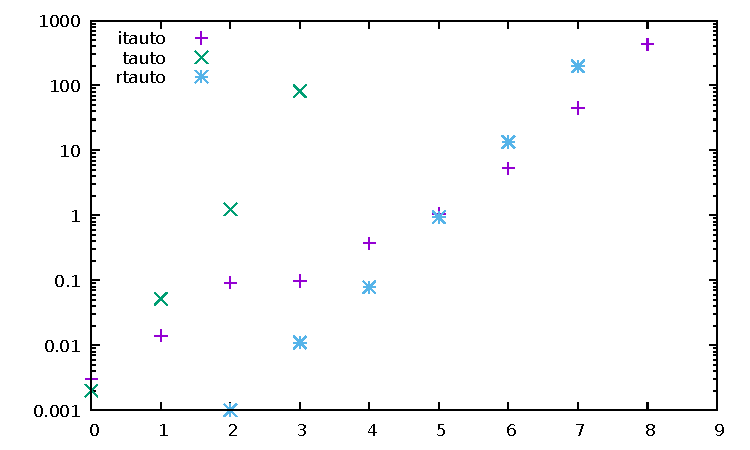
\includegraphics[width=0.45\linewidth]{images/pigeon_tac.pdf}}
  \qquad
  \subfloat[\centering Running time of type-checking.]
  {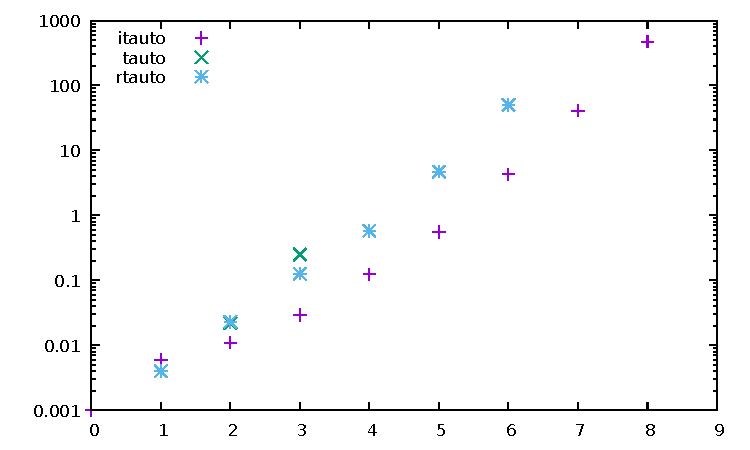
\includegraphics[width=0.45\linewidth]{images/pigeon_qed.pdf}}
  \caption{Pigeon Hole for \icoq{itauto}, \icoq{tauto} and \icoq{rtauto}}
  \label{fig:pigeon}
\end{figure}

\end{frame}

\begin{frame}[fragile]{Coq Benchmarks (1/2)}
  Replace all calls of \scoq{tauto}, \scoq{intuition tac} for\\
  \scoq{tac} $\in$ \{\scoq{idtac}, \scoq{assumption},
  \scoq{discriminate}, \scoq{congruence}, \scoq{lia}, \scoq{auto},
  \scoq{eauto} \}.\\
  \medskip
  
  \scoq{itauto} solves almost every goals but \dots
  \begin{itemize}
  \item Some goals are outside the pure quantifier-free fragment
\begin{minted}{Coq}
Goal true = true <-> (Z -> (False <-> False)).
Proof. Fail itauto congruence.
       itauto (itauto congruence). Qed.
\end{minted}
  \item The leaf tactic (sometimes) needs to be strengthen
    \begin{itemize}
    \item \scoq{idtac} $\to$ \scoq{reflexivity}
    \item \scoq{discriminate} $\to$ \scoq{congruence}
    \end{itemize}
  \end{itemize}

\end{frame}

\begin{frame}[fragile]{Coq Benchmarks (2/2)}
  Tested on two consequent developments: CompCert, Bedrock2\\
  (Sucessful runs)
  \bigskip
  
  \begin{tabular}{|l|c|c|c|c|}
    \hline
    & \#goals & \%faster & \%equal & \%slower \\
    \hline
    Bedrock2  & 1621   &   13   &   55    &   32     \\
    \hline
    CompCert  & 924    &   16   &   55    &   29      \\
    \hline
  \end{tabular}
  \bigskip
  
  \begin{itemize}
  \item  For Bedrock2, slowdown of 0.6
  \item  For CompCert, speed-up of 2.4\\
    16\% are solved 20 times faster!
  \end{itemize}

  Benchmarks are inconclusive\dots\\
  No clear suspect yet\dots
  
\end{frame}

\begin{frame}{Related Work}
  \begin{itemize}
  \item External SMT provers \emph{e.g.} SMTCoq\\
    classic logic, not extensible
  \item Reflexive (classic) SAT solver in Coq [Lescuyer, Conchon]
    \begin{itemize}
    \item CNF \checkmark
    \item Intuitionistic \xmark
    \item Hash-consing \xmark
    \item Lazy Unit Propagation \xmark
    \item Backjumping \xmark
    \item Theory   \xmark
    \end{itemize}
  \item Formalisation of SAT [Blanchette, Lamich, Fleury]
    \begin{itemize}
    \item Reflexive \xmark
    \item Intuitionistic \xmark
    \item Theory \xmark
    \item 2-watched \checkmark
    \item clause learning \checkmark
    \item imperative \checkmark
    \end{itemize}
  \end{itemize}
  
\end{frame}

\begin{frame}{Conclusion}
  Core of SMT solver
  \begin{itemize}
  \item Hash-consing
  \item CNF
  \item Backjumping
  \item Theory as a tactic
  \end{itemize}
  Missing features
  \begin{itemize}
  \item Clause learning (à la Cdcl)
  \item 2-watched literals 
  \item Imperative arrays
  \item à la Nelson-Oppen theory combination
  \end{itemize}
  \bigskip
  Try it out \url{https://gitlab.inria.fr/fbesson/itauto}\footnote{Happy user of the Patricia Trie library of Alix Trieu}
  
\end{frame}



\bibliographystyle{plainnat}
\bibliography{biblio}


\end{document}


%%% Local Variables:
%%% mode: latex
%%% TeX-engine: default
%%% TeX-command-extra-options: "-shell-escape"
%%% TeX-master: t
%%% End:


